\documentclass{article}

\usepackage{amsmath,amsfonts,amsthm,amssymb,amsopn,bm}
\usepackage[margin=.9in]{geometry}
\usepackage{graphicx}
\usepackage{url}
\usepackage[usenames,dvipsnames]{color}
\usepackage{fancyhdr}
\usepackage{multirow}
\newcommand{\field}[1]{\mathbb{#1}}
\newcommand{\1}{\mathbf{1}}
\newcommand{\E}{\mathbb{E}} 
\renewcommand{\P}{\mathbb{P}}
\newcommand{\R}{\field{R}} % real domain
% \newcommand{\C}{\field{C}} % complex domain
\newcommand{\F}{\field{F}} % functional domain

\newcommand{\T}{^{\textrm T}} % transpose

\def\diag{\text{diag}}

%% operator in linear algebra, functional analysis
\newcommand{\inner}[2]{#1\cdot #2}
\newcommand{\norm}[1]{\left\|#1\right\|}
\newcommand{\twonorm}[1]{\|#1\|_2^2}
% operator in functios, maps such as M: domain1 --> domain 2
\newcommand{\Map}[1]{\mathcal{#1}}
\renewcommand{\theenumi}{\alph{enumi}} 

\newcommand{\Perp}{\perp \! \! \! \perp}

\newcommand\independent{\protect\mathpalette{\protect\independenT}{\perp}}
\def\independenT#1#2{\mathrel{\rlap{$#1#2$}\mkern2mu{#1#2}}}
\newcommand{\vct}[1]{\boldsymbol{#1}} % vector
\newcommand{\mat}[1]{\boldsymbol{#1}} % matrix
\newcommand{\cst}[1]{\mathsf{#1}} % constant
\newcommand{\ProbOpr}[1]{\mathbb{#1}}
\newcommand{\points}[1]{\small\textcolor{magenta}{\emph{[#1 points]}} \normalsize}
\date{{}}

\setlength\parindent{0px}

\begin{document}
\title{Homework \#0}
\author{\normalsize{Spring 2020, CSE 446/546: Machine Learning}\\
\normalsize{Prof. Kevin Jamieson and Prof. Jamie Morgenstern} \\
\normalsize{Due: 4/8/19  11:59 PM}\\
\normalsize{A: 37 points. B: 3 points}}
\maketitle


\section*{Probability and Statistics}
A.1 \points{2} (Bayes Rule, from Murphy exercise 2.4.) After your yearly checkup, the doctor has bad news and good news. The bad news is that you tested positive for a serious disease, and that the test is 99\% accurate (i.e., the probability of testing positive given that you have the disease is 0.99, as is the probability of testing negative given that you dont have the disease). The good news is that this is a rare disease, striking only one in 10,000 people. What are the chances that you actually have the disease? (Show your calculations as well as giving the final result.)\\

A.2 For any two random variables $X,Y$ the \emph{covariance} is
  defined as
  $\text{Cov}(X,Y)=\E[(X-\E[X])(Y-\E[Y])]$. You may assume $X$ and $Y$
  take on a discrete values if you find that is easier to work with.
\begin{enumerate}
\item \points{1} If $\E[Y|X=x] = x$ show that $\text{Cov}(X,Y) = \E[(X-\E[X])^2]$.  
\item \points{1} If $X,Y$ are independent show that $\text{Cov}(X,Y)=0$.
\end{enumerate}


A.3 Let $X$ and $Y$ be independent random variables with PDFs given by $f$ and $g$, respectively. Let $h$ be the PDF of the random variable $Z = X+Y$.
\begin{enumerate}
	\item \points{2} Show that $h(z) = \int_{-\infty}^\infty f(x) g( z - x ) d x $.  (If you are more comfortable with discrete probabilities, you can instead derive an analogous expression for the discrete case,  and then you should give a one sentence explanation as to why your expression is analogous to the continuous case.).
	\item \points{1} If $X$ and $Y$ are both independent and uniformly distributed on $[0,1]$ (i.e. $f(x)=g(x)=1$ for $x \in [0,1]$ and $0$ otherwise) what is $h$, the PDF of $Z=X+Y$?
\end{enumerate}

A.4 \points{1} A random variable $X \sim \mathcal{N}(\mu, \sigma^2)$ is Gaussian distributed with mean $\mu$ and variance $\sigma^2$. Given that for any $a,b \in \R$, we have that $Y = aX + b$ is also Gaussian, find $a,b$ such that $Y \sim \mathcal{N}(0,1)$.\\

A.5 \points{2} For a random variable $Z$, its mean and variance are defined as $\E[Z]$ and $\E[(Z-\E[Z])^2]$, respectively.
Let $X_1,\dots,X_n$ be independent and identically distributed random variables, each with mean $\mu$ and variance $\sigma^2$. 
If we define $\widehat{\mu}_n = \frac{1}{n} \sum_{i=1}^n X_i$, what is the mean and variance of $\sqrt{n}(\widehat{\mu}_n - \mu)$?\\

A.6 If $f(x)$ is a PDF, the cumulative distribution function (CDF)
  is  defined as $F(x) = \int_{-\infty}^x f(y) dy$.  For any function
  $g : \R \rightarrow \R$ and random variable $X$ with PDF $f(x)$,
  recall that the expected value of $g(X)$ is defined as
  $\E[g(X)] = \int_{-\infty}^\infty g(y) f(y) dy$. For a boolean event
  $A$, define $\1\{ A \}$ as $1$ if $A$ is true, and $0$
  otherwise. Thus, $\1\{ x \leq a \}$ is $1$ whenever $x \leq a$ and
  $0$ whenever $x > a$.  Note that $F(x) = \E[\1\{X \leq x\}]$.  Let
  $X_1,\dots,X_n$ be \emph{independent and identically distributed}
  random variables with CDF $F(x)$.  Define
  $\widehat{F}_n(x) = \frac{1}{n} \sum_{i=1}^n \1\{X_i \leq
  x\}$. Note, for every $x$,
  that $\widehat{F}_n(x)$ is an \emph{empirical estimate} of  $F(x)$.
  You may use your answers to the previous problem.
  \begin{enumerate}
  \item \points{1} For any $x$, what is $\E[ \widehat{F}_n(x) ]$?
  \item \points{1} For any $x$, the variance of $\widehat{F}_n(x)$ is $\E[ ( \widehat{F}_n(x) -
    F(x) )^2 ]$.  Show that $\textrm{Variance}(\widehat{F}_n(x)) = \frac{F(x)(1-F(x))}{n}$. \\
%    (Hint: Consider what independence implies.)
  \item \points{1} Using your answer to b, show that
    for all $x\in \R$, we have  $\displaystyle \E[ ( \widehat{F}_n(x) - F(x) )^2 ] \leq \tfrac{1}{4n}$.  
  \end{enumerate} 

B.1  \points{1} Let $X_1,\dots,X_n$ be $n$ independent and identically distributed random variables drawn unfiromly at random from $[0,1]$. If $Y = \max\{X_1,\dots,X_n\}$ then find $\E[Y]$.\\


\section*{Linear Algebra and Vector Calculus}
A.7 (Rank) Let $A = \begin{bmatrix} 1 & 2 & 1 \\ 1 & 0 & 3 \\ 1 & 1 & 2 \end{bmatrix}$ and $B = \begin{bmatrix} 1 & 2 & 3 \\ 1 & 0 & 1 \\ 1 & 1 & 2 \end{bmatrix}$.
For each matrix $A$ and $B$,
\begin{enumerate} 
	\item \points{2} what is its rank? 
	\item \points{2} what is a (minimal size) basis for its column span?
\end{enumerate}

A.8 (Linear equations) Let $A = \begin{bmatrix} 0 & 2 & 4 \\ 2 & 4 & 2 \\ 3 & 3 & 1 \end{bmatrix}$, $b = \begin{bmatrix} -2 & -2 & -4 \end{bmatrix}^T$, and $c=\begin{bmatrix} 1 & 1 & 1 \end{bmatrix}^T$.
\begin{enumerate}
	\item \points{1} What is $Ac$?
	\item \points{2} What is the solution to the linear system $Ax = b$? (Show your work).
\end{enumerate}

A.9 (Hyperplanes) Assume $w$ is an $n$-dimensional vector and $b$ is a scalar. A hyperplane in $\R^n$ is the set $\{x : x\in \R^n,\text{ s.t. } w^T x + b = 0\}$.
\begin{enumerate}
	\item \points{1} ($n=2$ example) Draw the hyperplane for $w=[-1,2]^T$, $b=2$? Label your axes.
	\item \points{1} ($n=3$ example) Draw the hyperplane for $w=[1,1,1]^T$, $b=0$? Label your axes.
	\item \points{2} Given some $x_0 \in \R^n$, find the \emph{squared distance} to the hyperplane defined by $w^T x + b=0$.
	In other words, solve the following optimization problem:
	\begin{align*}
	\min_x& \|x_0 - x \|^2\\
	\text{s.t. }&w^Tx +b = 0
	\end{align*}
	(Hint: if $\widetilde{x}_0$ is the minimizer of the above problem, note that $\| x_0 - \widetilde{x}_0 \| = | \frac{w^T(x_0 - \widetilde{x}_0)}{\|w\|} |$. What is $w^T \widetilde{x}_0$?)
\end{enumerate} 

A.10 For possibly non-symmetric $\mat{A}, \mat{B} \in \R^{n \times n}$ and $c \in \R$, let $f(x, y) = x^T \mat{A} x + y^T \mat{B} x + c$. Define $\nabla_z f(x,y) = \begin{bmatrix} \frac{\partial f(x,y)}{\partial z_1} & \frac{\partial f(x,y)}{\partial z_2} & \dots & \frac{\partial f(x,y)}{\partial z_n} \end{bmatrix}^T$.  
\begin{enumerate}
	\item \points{2} Explicitly write out the function $f(x, y)$ in terms of the components $A_{i,j}$ and $B_{i,j}$ using appropriate summations over the indices.
	\item \points{2} What is $\nabla_x f(x,y)$ in terms of the summations over indices \emph{and} vector notation?
	\item \points{2} What is $\nabla_y f(x,y)$ in terms of the summations over indices \emph{and} vector notation?
\end{enumerate}

B.2 \points{1} The \textit{trace} of a matrix is the sum of the diagonal entries; $Tr(A) = \sum_i A_{ii}$. If $A\in\mathbb{R}^{n\times m}$ and $B\in\mathbb{R}^{m\times n}$, show that $Tr(AB) = Tr(BA)$.\\

B.3 \points{1} Let $v_1,\dots,v_n$ be a set of non-zero vectors in $\mathbb{R}^d$. Let $V = [v_1,\dots,v_n]$ be the vectors concatenated. 
    \begin{enumerate}
        \item What is the minimum and maximum rank of $\sum_{i=1}^n v_i v_i^T$?
        \item What is the minimum and maximum rank of $V$?
        \item Let $A \in \mathbb{R}^{D \times d}$ for $D > d$. What is the minimum and maximum rank of $\sum_{i=1}^n (A v_i) (A v_i)^T$?
        \item What is the minimum and maximum rank of $AV$? What if $V$ is rank $d$?
    \end{enumerate}

\section*{Programming}

A.11 For the $A, b, c$ as defined in Problem 8, use
  NumPy to compute (take a screen shot of your answer):
  \begin{enumerate}
  \item \points{2} What is $A^{-1}$?
  \item \points{1} What is $A^{-1}b$? What is $Ac$?
  \end{enumerate}  


A.12 \points{4} Two random variables $X$ and $Y$ have equal
  distributions if their CDFs, $F_X$ and $F_Y$, respectively, are
  equal, i.e. for all $x$, $ |F_X(x) - F_Y(x)| = 0$. 
The central limit theorem says that the sum of $k$ independent,
zero-mean, variance-$1/k$ random variables converges to a (standard) Normal distribution as $k$ goes off to infinity.  
We will study this phenomenon empirically (you will use the Python packages Numpy and Matplotlib). 
Define $Y^{(k)} = \frac{1}{\sqrt{k}} \sum_{i=1}^k B_i$ where each $B_i$ is equal to $-1$ and $1$ with equal probability.
From your solution to problem 5, we know that $\frac{1}{\sqrt{k}} B_i$ is zero-mean and has variance $1/k$.
\begin{enumerate}
\item For $i=1,\dots,n$ let $Z_i \sim \mathcal{N}(0,1)$. If
  $F(x)$ is the true CDF from which each $Z_i$ is drawn (i.e.,
  Gaussian) and $\widehat{F}_n(x) = \frac{1}{n} \sum_{i=1}^n
  \1\{ Z_i \leq x)$, use the answer to problem 1.5  above to choose
  $n$ large enough such that, for all $x \in \R$, $ \sqrt{\E[
    (\widehat{F}_n(x)-F(x))^2 ]} \leq 0.0025$, and plot
  $\widehat{F}_n(x)$ from $-3$ to $3$. \\(Hint: use
  \texttt{Z=numpy.random.randn(n)} to generate the random
  variables, and \texttt{import matplotlib.pyplot as plt};\\
  \texttt{plt.step(sorted(Z), np.arange(1,n+1)/float(n))} to
  plot). 
\item For each $k \in \{1, 8, 64, 512\}$ generate $n$
  independent copies $Y^{(k)}$ and plot their empirical CDF on
  the same plot as part a.\\ (Hint: 
  $\texttt{np.sum(np.sign(np.random.randn(n,
    k))*np.sqrt(1./k), axis=1)}$ generates $n$ of the
  $Y^{(k)}$ random variables.) 
\end{enumerate}
Be sure to always label your axes. 
Your plot should look something like the following (Tip: checkout \texttt{seaborn} for instantly better looking plots.)

\begin{center}
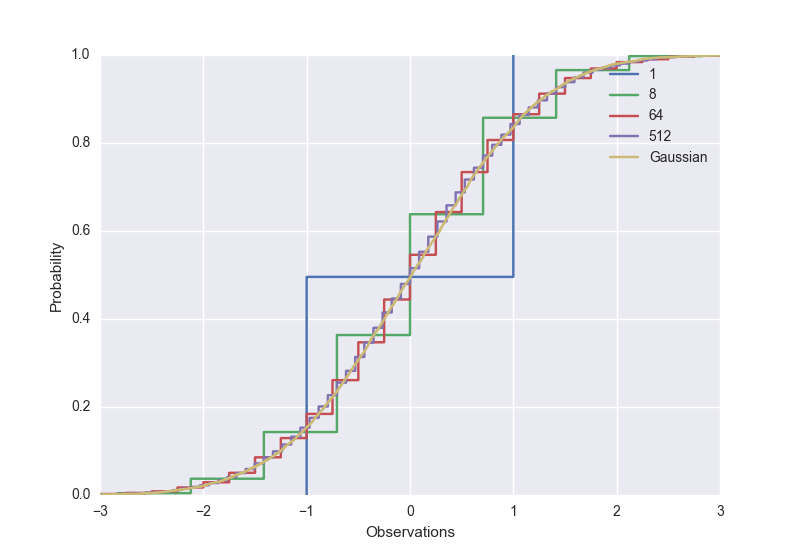
\includegraphics[width=4in]{full.png}
\end{center} 




\end{document}
